\documentclass[12pt]{article}
\usepackage[normalem]{ulem}
\usepackage{graphicx, multirow}
\usepackage{amsmath, array}
\usepackage{fancyheadings, lastpage}
\usepackage{pdflscape ,anyfontsize}
\usepackage{longtable}
\usepackage{changepage}
\usepackage[a4paper]{geometry}
\renewcommand{\headrulewidth}{0pt}
\lhead{Group Project 07 – Project Plan}
\rhead{(Release) -Version 2.3}
\lfoot{Aberystwyth University / Computer Science}
\cfoot{}
\rfoot{\thepage{}  of  \pageref{LastPage}}
\begin{document}
\pagestyle{fancy}
\begin{flushleft}
\rule[0.5cm]{13.8cm}{0.02cm}
\end{flushleft}
{\fontsize{20}{20}\selectfont \textbf {\centerline{Group Project 07 Project Plan}}}
\begin{flushleft}
\rule[0.5cm]{13.8cm}{0.02cm}
\end{flushleft}

\begin{tabular}{ l l }

\\ \multirow{1}{*}{\textit{Authors: }} & Mosopefoluwa David Adejumo \\  & Ryan Gouldsmith \\
& Harry Flynn Buckley \\ & Zack Lott \\ & Mark Radcliffe Pitman \\ & Jack Alexander Reeve \\ & Mark Alexander Smith \\ &Martin Vasilev Zokov \\ & Maciej Wojciech Dobrzanski \\
\\ \multirow{1}{*}{\textit{Config ref: }} & SE\_07\_PM\_01 \\
\\ \multirow{1}{*}{\textit{Date} } & \today \\
\\ \multirow{1}{*}{\textit{Version}} & 2.3 \\ 
\\ \multirow{1}{*}{\textit{Status}} & Release \\

\end{tabular}


\vspace{3.2cm}
\hfill\begin{minipage}{\dimexpr\textwidth-0.3cm}
Department of Computer Science \\
Aberystwyth University \\
Aberystwyth \\
Ceredigion\\
SY23 3DB \\
Copyright \small{\copyright}\\ Aberystwyth University 2013
\end{minipage}



\newpage
\tableofcontents{}
\newpage
\section{INTRODUCTION}
\subsection{Purpose}
This document displays how the project will be completed and any risks involved.  It outlines the requirements specified by the client as a series of documents.
\subsection{Scope}
This document should be read by all members of the group. It contains a list of tasks, the schedule and risks involved in the project. It details what the application and server will be required to do. It also gives an overview of the whole software - the Use Case diagrams, UML diagrams, the UI of the website and the navigation overview of Android application and the website. The Gantt chart gives an idea of our milestones and describes what tasks are assigned to every member of the group. The document doesn't give any specifics about the classes in the application, doesn't cover any information about the database connection and it doesn't provide information about the website. These will be covered in the design specification.
\subsection{Objective}
\begin{itemize}
\item List the platforms to be used for the project
\item Provide a task schedule for the project 
\item Provide a description of how the application and website will be used.
\item Provide a list of risks and how to reduce their effects
\item Provide an idea of the UI for the Android application and the website
\item Provide a description of how the application and website can be navigated
\end{itemize}
\newpage
\section{PROJECT OVERVIEW}
The proposed system is an application running on the Android operating system that will be used to record walks for a particular user. The application will allow the user to start a recording of a new walk and add points of interest to that walk and save the walk.
The website will allow the user to view the walks they uploaded, with all the information associated with it, like points of interest with the photos and descriptions on the map, short and long description of the walk itself and the entire path the user recorded.
\subsection{Platforms}
\subsubsection{Android}
As stated by the client, the operating system used will be Android. This will be developed for mobile devices. The operating system version will be 4.2. This is because we have a few devices running on that operating system, so it is just the most convenient one.
\subsubsection{HTML 5}
The website will be built using HTML 5 alongside CSS 2 and CSS 3. This will allow the latest version of HTML to be used for the website. We are going to use Google Maps, which requires the latest version.
\subsubsection{PHP}
PHP will be used to handle the communication between the mobile device and the server. It will be run server side and is understood to a working level by the web programmers.
\subsubsection{MySQL}
The database will be built using MySQL. It shall store information about each walk and the walk themselves. Information stored will include all points of interest added, their associated long and short descriptions and any pictures taken.
\subsubsection{Google Maps API}
This API gives us all the features we need. OpenSpace API gives some additional ones like offline use, but we decided that it is not really required in our project, so we decided that Google Maps is just easier to work on. 
\subsection{Target Audience}
This application is aimed at Second Year Computer Science students. Precautions had to be taken while designing the user interface to prevent the user from having to navigate through too many screens. 
\subsection{System Overview}
\begin{figure}[htp]
\centering
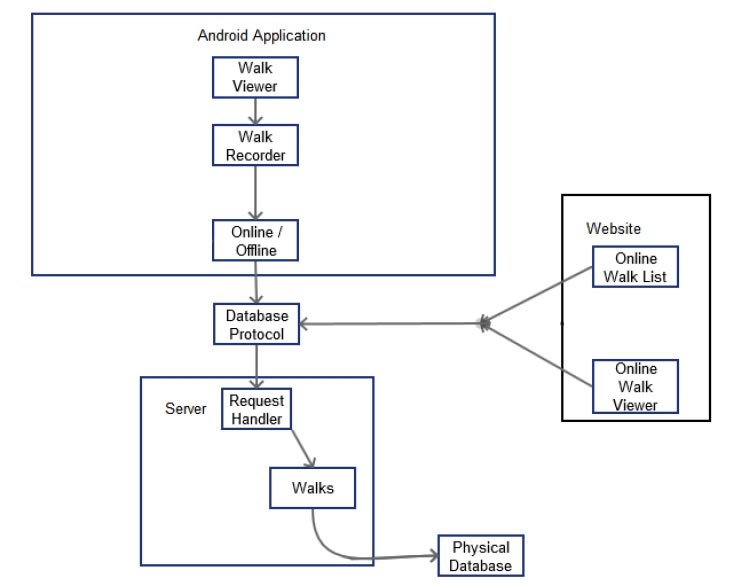
\includegraphics[scale=0.50]{Project_Plan/docs/ProjectPlan2-3.jpg}
\caption{System Overview}
\label{System Overview}
\end{figure}
\subsubsection{Android Application}
This is the application. All modules here are running on the mobile device
\subsubsection{Online Offline}
This module handles the location where data is stored. If the user is not connected to the internet they receives an error message saying that they won't be able to upload the walk.
\subsubsection{Walk Screen}
This module handles the displaying options about the walk, like cancelling it, adding points of interest or uploading it.
\subsubsection{Walk Recorder}
This module handles the storage of points of interest, the time taken for a walk and the walks location during recording.
\subsubsection{Database Protocol}
This module handles the conversion of database request to their required language such as from POST to HTTP for the website.
\subsubsection{Server}
This is the server that handles all requests between the database, website and android application
\subsubsection{Request Handler}
\par{This module deals with linking data between users}
\subsubsection{Walks}
This module handles the retrieval and presentation of the walks uploaded by the user.
\subsubsection{Physical Database}
\par{This is the machine where all request are handled}
\subsubsection{Website}
\par{This module serves as the control for everything on the website}
\subsubsection{Online Walk List}
This module handles all lists being displayed to anyone on the website.
\subsubsection{Online Walk Viewer}
This module handles the conversion of data into visual form for browser based viewing of walks.
\newpage
\section{USE CASE}
\subsection{Android}
\begin{figure}[htp]
\centering
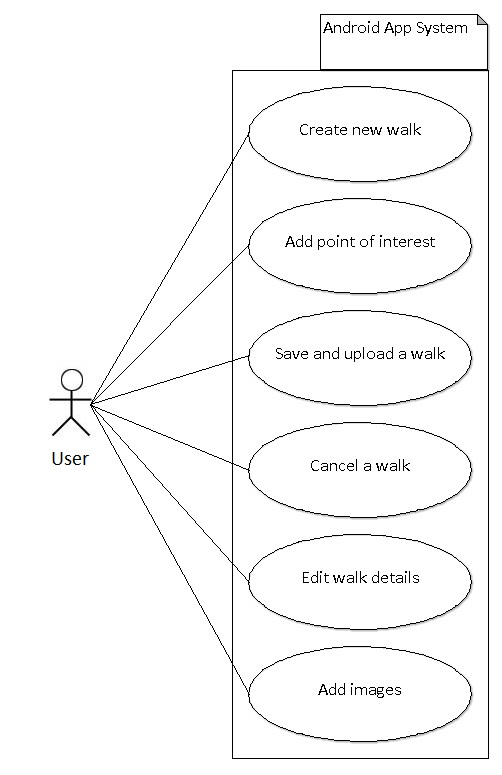
\includegraphics[scale=0.50]{Project_Plan/docs/Android_use_case_final.jpg}
\caption{Android Use-Case diagram}
\label{Android Use-Case Diagram}
\end{figure}
\subsection{Website}
\clearpage
\begin{figure}[htp]
\centering
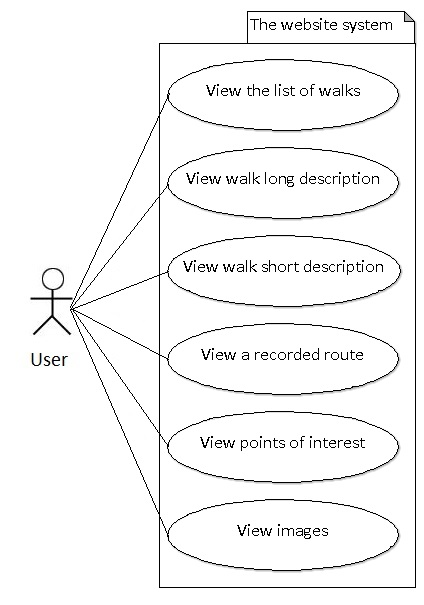
\includegraphics[scale=0.60]{Project_Plan/docs/website_use_case.jpg}
\caption{Website Use-Case Diagram}
\label{Website Use-Case Diagram}
\end{figure}
\subsection{Interaction System}
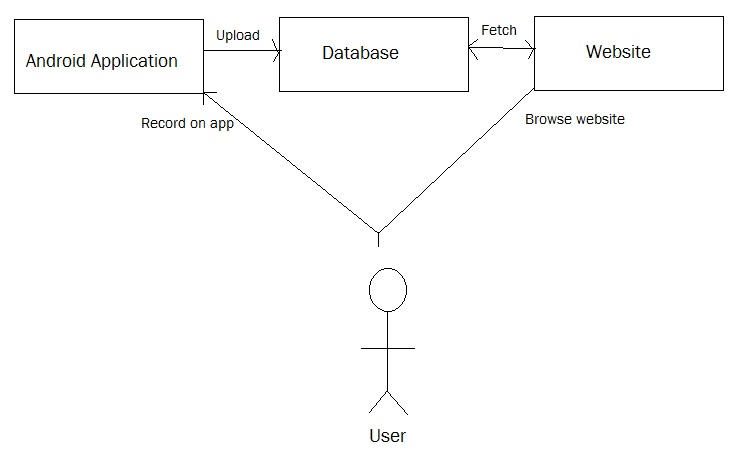
\includegraphics[scale=0.60]{Project_Plan/docs/system_interaction.jpg}
\par{The diagram above represents the interaction of the whole system. The user interacts with both Android application and the website. The walks recorded by the user along with all the other information like description and the photos, are stored in the database and can be easily accessed later via the website. All uploads are stored in the database for the website to retrieve
The Android application uploads walks to the server, which deals with the information and inserts it appropriately in the database. The Android application does not have a direct link to the website.The website also pulls a list of walks from the database. The website will also list all the information associated to one singular walks, such as Long description, short description, any pictures. This will then be displayed appropriately on the website.}
\subsection{Descriptions}
\clearpage
\setlength\LTleft{-1cm}
\begin{longtable}{|p{2cm}|p{3cm}|p{10cm}|}
\hline
	Diagram Name & Use case name  & Description \\
\hline

 \multirow{4}{*}{Android} & \multicolumn{1}{|p{3cm}|}{Create new walk} & \multicolumn{1}{|p{10cm}|}{Allows the user to start recording a new walk} \\\cline{2-3} & \multicolumn{1}{|p{3cm}|}{Add a point of interest
} & \multicolumn{1}{|p{10cm}|}{The user must add points of interest on the walk. This includes a short description, an optional long description and optional images. A timestamp is automatically taken when a point of interest is saved}
\\\cline{2-3} & \multicolumn{1}{|p{3cm}|}{Save and upload a walk} & \multicolumn{1}{|p{10cm}|}{When the user has finished their walk they will click the finish the walk button, this will then upload the walk to the server where it will be processed.}
\\\cline{2-3} & \multicolumn{1}{|p{3cm}|}{Cancel a walk} & \multicolumn{1}{|p{10cm}|}{If the user wishes to end their walk then they can click the cancel button. This will cancel any recorded data associated with the current walk.}
\\\cline{2-3} & \multicolumn{1}{|p{3cm}|}{Edit walk details} & \multicolumn{1}{|p{10cm}|}{The user will be able to edit any information associated with the current walk. This could be a point of interest, or the title of the whole walk. The information about the walk, in which they're editing, has to be shown to the user.}
\\\cline{2-3} & \multicolumn{1}{|p{3cm}|}{Add point of interest} & \multicolumn{1}{|p{10cm}|}{The user can add points of interest. These are locations with descriptions with or without images}
\\\cline{2-3} & \multicolumn{1}{|p{3cm}|}{Add POI Images} & \multicolumn{1}{|p{10cm}|}{The user can take a picture of a location and add it to the walk. Alternatively, they can add a picture from their photo library. The user should be also able to upload multiple images to any given point of interest.}
\\\cline{2-3} & \multicolumn{1}{|p{3cm}|}{Add POI Long Description} & \multicolumn{1}{|p{10cm}|}{The user can add a detailed description of a point of interest}
\\\cline{2-3} & \multicolumn{1}{|p{3cm}|}{Add POI Short Description} & \multicolumn{1}{|p{10cm}|}{The user can add a brief description summarising a point of interest}
\\\cline{2-3} & \multicolumn{1}{|p{3cm}|}{Add Walk Descriptions} & \multicolumn{1}{|p{10cm}|}{The user can add description both long and short to the walk and can be edited later}
\\\hline
 \multirow{4}{*}{Website} & \multicolumn{1}{|p{3cm}|}{View the list of walks} & \multicolumn{1}{|p{10cm}|}{This will show a list of the walks in the database that multiple user has uploaded to the server. They will be displayed in a list form on the website.} \\\cline{2-3} & \multicolumn{1}{|p{3cm}|}{View walk long description}& \multicolumn{1}{|p{10cm}|}{Once a walk has been selected from the list of walks it will tell the user what the long description associated to that walk is. This will also appear, in the google maps popup.}
\\\cline{2-3} & \multicolumn{1}{|p{3cm}|}{View walk short description}& \multicolumn{1}{|p{10cm}|}{Once a walk has been selected from the list of walks it will tell the user what the short description associated to that walk is. This will also appear, in the google maps popup.}
\\\cline{2-3} & \multicolumn{1}{|p{3cm}|}{View a recorded route}& \multicolumn{1}{|p{10cm}|}{When the user selects the walk from the list of walks screen, then it should show the user the route they have walked. This will be shown on the map as a trail. Each of the points of interest along the walk will be located with a marker.}
\\\cline{2-3} & \multicolumn{1}{|p{3cm}|}{View points of interest.}& \multicolumn{1}{|p{10cm}|}{When the user views the walk and it has a series of points of interests, they will be shown on the map as a marker value. The user will then be able to click on the marker; there will then be a popup showing the walk title, description for that POI. Along images inside the popup, this allows the option for multiple images.}
\\\cline{2-3} & \multicolumn{1}{|p{3cm}|}{View images.}& \multicolumn{1}{|p{10cm}|}{When the user selects a walk they will be able to see all the images associated with the walk on the side. If they wish to see where the images comes from, the images will be associated with a given marker on the map.}
\\\hline
\end{longtable}
\newpage
\section{ANDROID USER INTERFACE DESIGN}
\subsection{Start Screen}
\begin{figure}[htp]
\centering
\includegraphics[scale=0.40]{Project_Plan/android/main_screen_new.png}
\caption{Start Screen}
\label{Start Screen}
\end{figure}
Used as a filler screen before the user starts a walk. This screen may be replaced with a tutorial or help screen on first launch in future. \\\\
\textbf{\uline{NAVIGATION}}
\par{Start $\rightarrow$ New Walk Screen (Fig. 4.2)} 
\clearpage
\subsection{New Walk Screen}
\begin{figure}[htp]
\centering
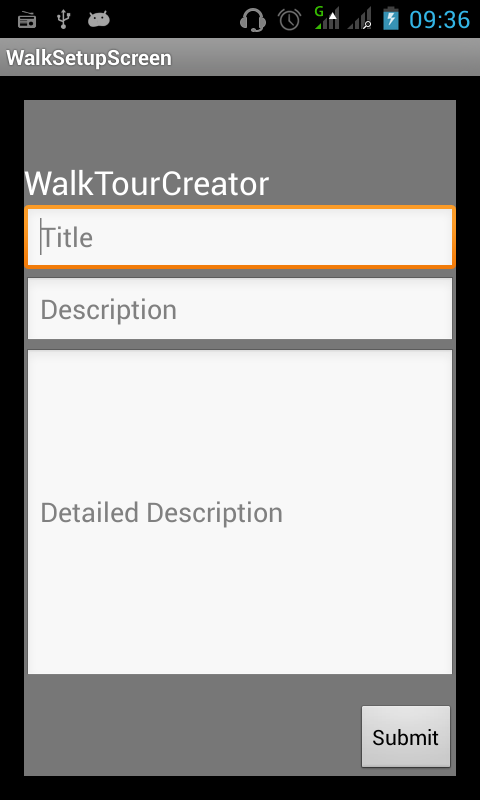
\includegraphics[scale=0.40]{Project_Plan/android/new_walk.png}
\caption{}
\label{}
\end{figure}
\par{This is the walk creation screen. It allows a short and long description to be added to a walk.  \\ \\}
\textbf{\uline{NAVIGATION}}
\par{Back $\rightarrow$ Main Menu (Fig. 4.1)}
\par{Start Walk $\rightarrow$ Recording Screen (Fig. 4.3)}
\clearpage
\subsection{Recording Screen}
\begin{figure}[htp]
\centering
\includegraphics[scale=0.40]{Project_Plan/android/walk_recording.png}
\caption{}
\label{}
\end{figure}
\par{This screen will give the user the option to edit the walk, add points of interest and finish or cancel walks. Recording will only begin when a GPS signal has been found. The user will receive a message to indicate recording has begun\\ \\}
\textbf{\uline{NAVIGATION}}
\par{Add POI $\rightarrow$ New Point of Interest Screen (Fig. 4.4)}
\par{Edit Walk $\rightarrow$ Edit Walk Information Screen (Fig 4.5)}
\par{Finish $\rightarrow$ Walk Complete Screen(Fig. 4.6)}
\par{Cancel Walk $\rightarrow$ Start screen without uploading walk (Fig 4.1)}
\subsection{New Point Of Interest}
\begin{figure}[htp]
\centering
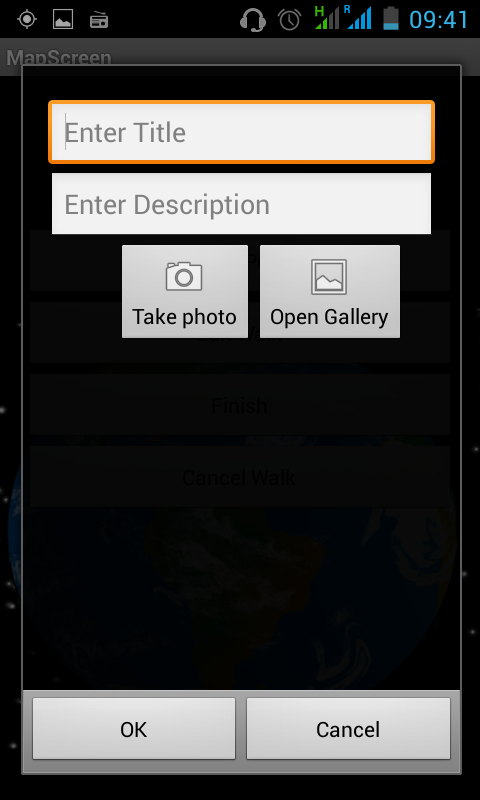
\includegraphics[scale=0.4]{Project_Plan/android/add_poi.png}
\caption{Add Point Of Interest}
\label{Add Point Of Interest}
\end{figure}
\par{This screen is used to add a point of interest. It will appear over the recording screen. Adding images will open a dialogue asking whether to go to the photo library or the camera app, allowing images to be added. Images will appear between the short and long description and can be removed from here. Pressing save stores the point of interest but can be removed later. \\ \\}
\textbf{\uline{NAVIGATION}}
\par{Cancel $\rightarrow$ Recording screen without saving(Fig. 4.3)}
\par{Add Image $\rightarrow$ Dialogue for Camera or Photo Library}
\par{Save $\rightarrow$ Recording screen with save (Fig. 4.3)}
\subsection{Edit Walk Information Screen}
\begin{figure}[htp]
\centering
\includegraphics[scale=0.40]{Project_Plan/android/edit_walk.png}
\caption{Edit Walk}
\label{Edit Walk}
\end{figure}
\par{This screen allows the user to edit the walk information}
\par{OK $\rightarrow$ Recording Screen with new details(Fig 4.3)}
\par{Cancel $\rightarrow$ Recording Screen without saving (Fig 4.3)}
\clearpage
\subsection{Walk Complete}
\begin{figure}[htp]
\centering
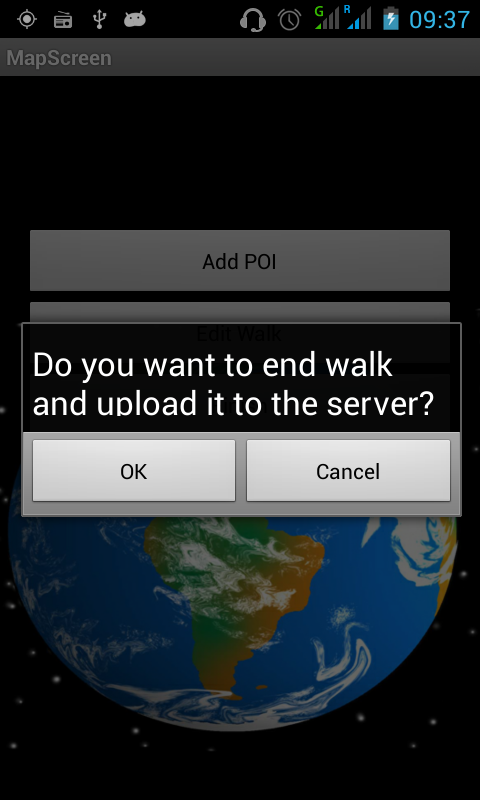
\includegraphics[scale=0.40]{Project_Plan/android/upload_walk.png}
\caption{Upload Walk}
\label{Upload Walk}
\end{figure}
\par{This screen allows the user to save a walk. If upload is pressed, the walk is saved then uploaded to the server provided the user is signed in. This screen should be unavailable if there are no points of interest to prevent uploading or saving an empty walk. IN future, this screen could show the time taken to complete a walk, the name of the walk, the number of points of interest added and the location of the walk. \\ \\}
\textbf{\uline{NAVIGATION}}
\par{Cancel $\rightarrow$ Recording Screen without uploading(Fig. 4.3)}
\par{OK $\rightarrow$ Start Screen (Fig. 4.1)}
\subsection{Cancel A Walk}
\begin{figure}[htp]
\centering
\includegraphics[scale=0.40]{Project_Plan/android/cancel_walk.png}
\caption{Cancel A Walk}
\label{Cancel A Walk}
\end{figure}
TODO
\newpage
\section{WEBSITE USER INTERFACE DESIGN}
\subsection{Home Page}

\begin{figure}[htp]
\centering

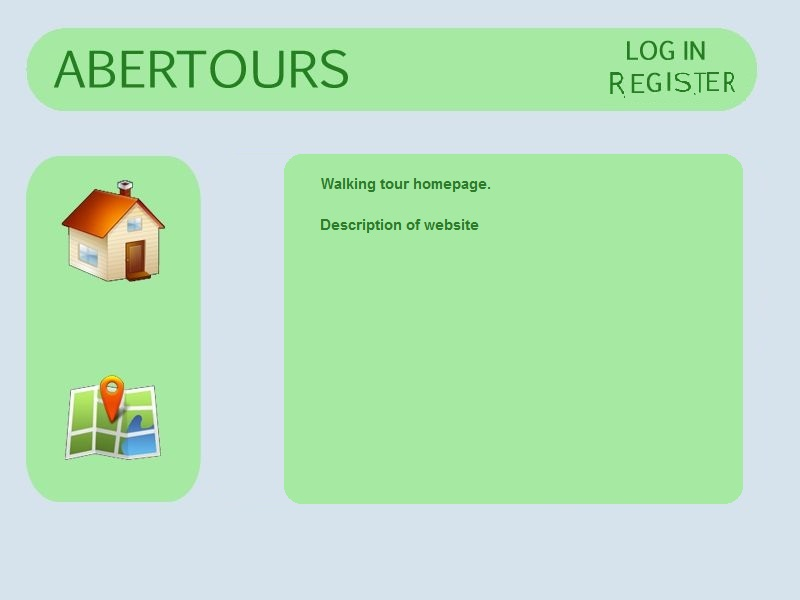
\includegraphics[scale=0.60]{Project_Plan/Web/homepage_01.jpg}
\caption{Website Home Page}
\label{Website Home Page}
\end{figure}
\par{This is the homepage of the website. From here the user can find information about the application page and can view walks. \\ \\}
\textbf{\uline{NAVIGATION}}
\par{View Walks $\rightarrow$ View Walks Page (Fig. 5.2)}
\clearpage
\subsection{View Walks Page}
\begin{figure}[htp]
\centering
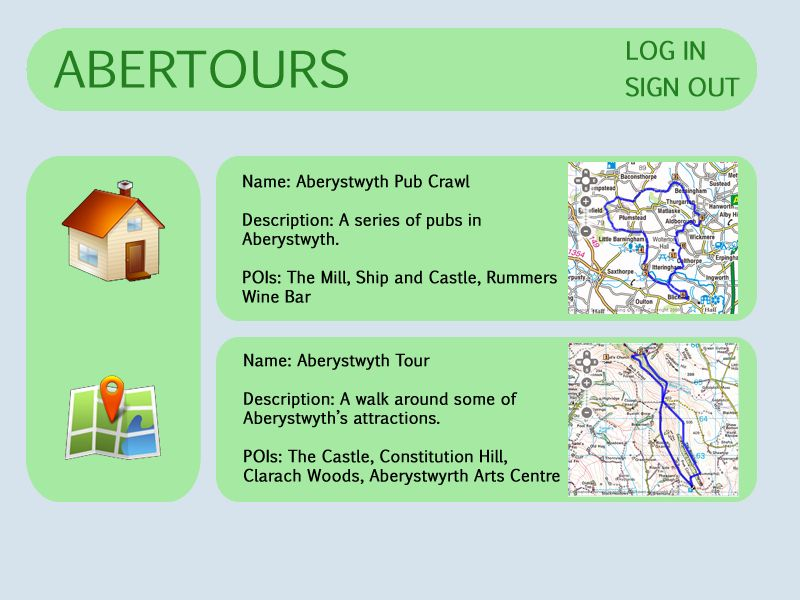
\includegraphics[scale=0.60]{Project_Plan/Web/Your_Tours_Page_01.jpg}
\caption{View Walks Page}
\label{View Walks Page}
\end{figure}
\par{The user can view all uploaded walks via this screen. From here the user can see a small map overview of the walk and the short description of the points of interest. \\ \\}
\textbf{\uline{NAVIGATION}}
\par{Click on Walk $\rightarrow$ Walk Page (Fig. 5.3)}
\par{Home $\rightarrow$ Home Page (Fig. 5.1)}
\clearpage
\subsection{Walk Page}
\begin{figure}[htp]
\centering
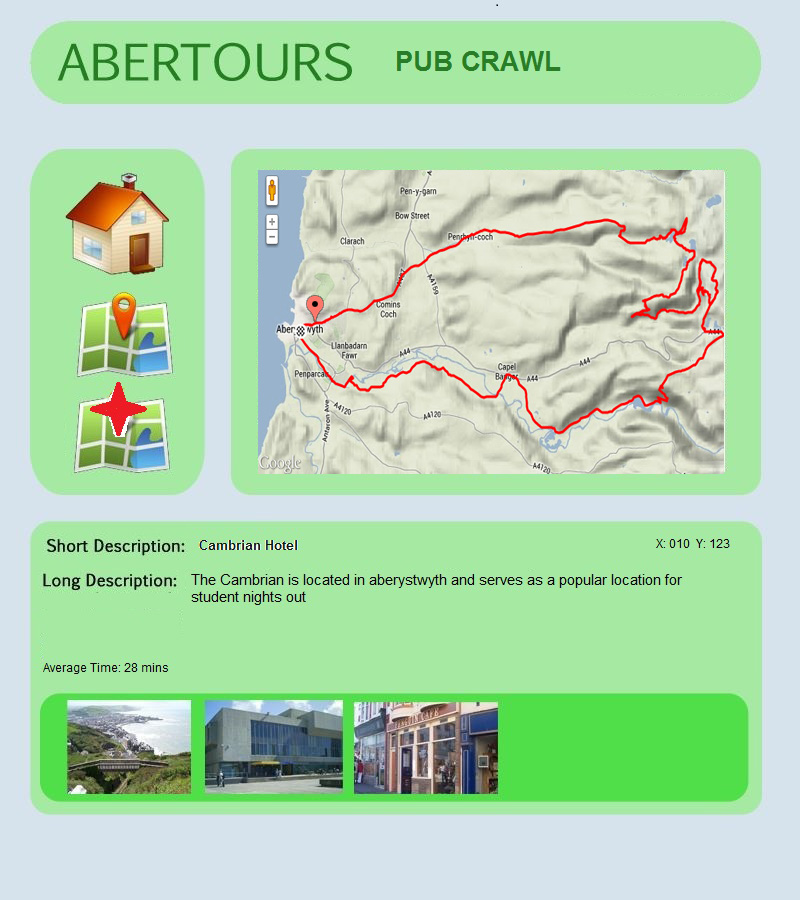
\includegraphics[scale=0.50]{Project_Plan/Web/poi_selected_page_01_copy.jpg}

\caption{Walk Page }
\label{Walk Page}
\end{figure}
\par{This page displays a map overview of the walk, the average time taken to complete the walk and the long and short descriptions. The images from every point of interest are displayed at the bottom of the screen. \\ \\}
\textbf{\uline{NAVIGATION}}
\par{Click on Image $\rightarrow$ Point of Interest Image Page (Fig. 5.4)}
\par{Click Pin on Map $\rightarrow$ Point of Image Selected Page (Fig. 5.5)}
\par{View Walks $\rightarrow$ View Walks Page (Fig. 5.2)}
\par{Home $\rightarrow$ Home Page (Fig. 5.1)}
\clearpage
\subsection{Point Of Interest Selected Page}

\begin{figure}[htp]
\centering
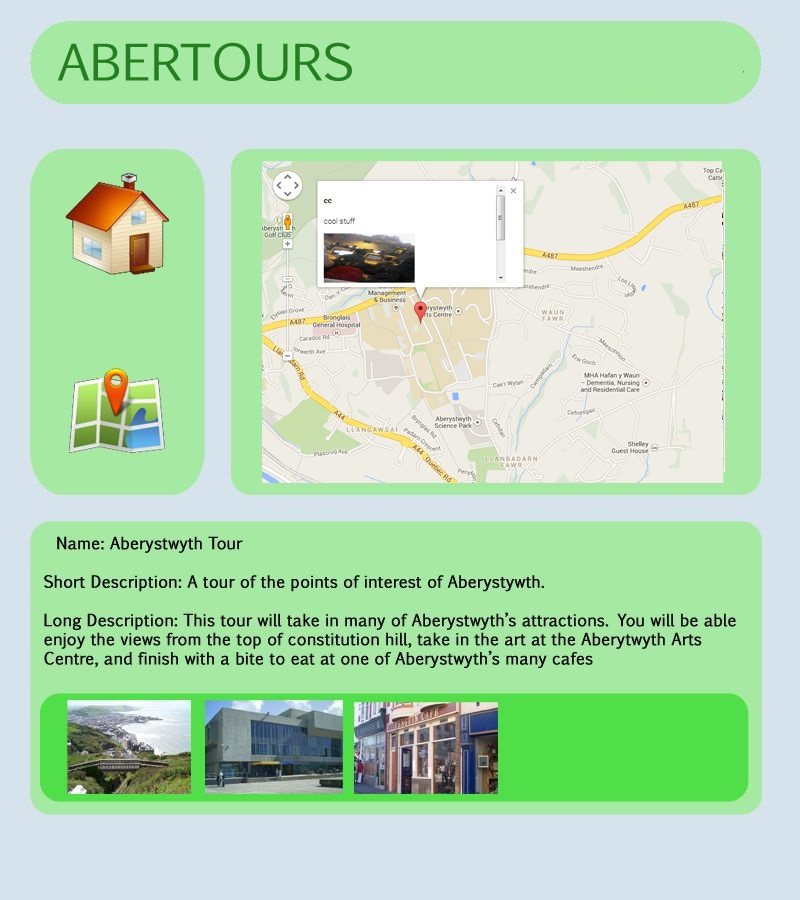
\includegraphics[scale=0.50]{Project_Plan/Web/new_map_copy2.jpg}
\caption{Point Of Interest Selected}
\label{Point Of Interest Selected}
\end{figure}
\par{Clicking on a pin on the map opens this page. The selected pin is also highlighted. The page displays the average time taken from the start of the walk to arrive at this point of interest. If there are any images taken from this point of interest, the user is can view them.\\ \\}
\textbf{\uline{NAVIGATION}}
\par{Click on Map $\rightarrow$ Walk Page (Fig. 5.3)}
\par{Click Pin on Map $\rightarrow$ Point of Image Selected Page (Fig. 5.5)}
\par{View Walks $\rightarrow$ View Walks Page (Fig. 5.2)}
\par{Home $\rightarrow$ Home Page (Fig. 5.1)}
\clearpage
\subsection{Point Of Interest Image Page}
\begin{figure}[htp]
\centering
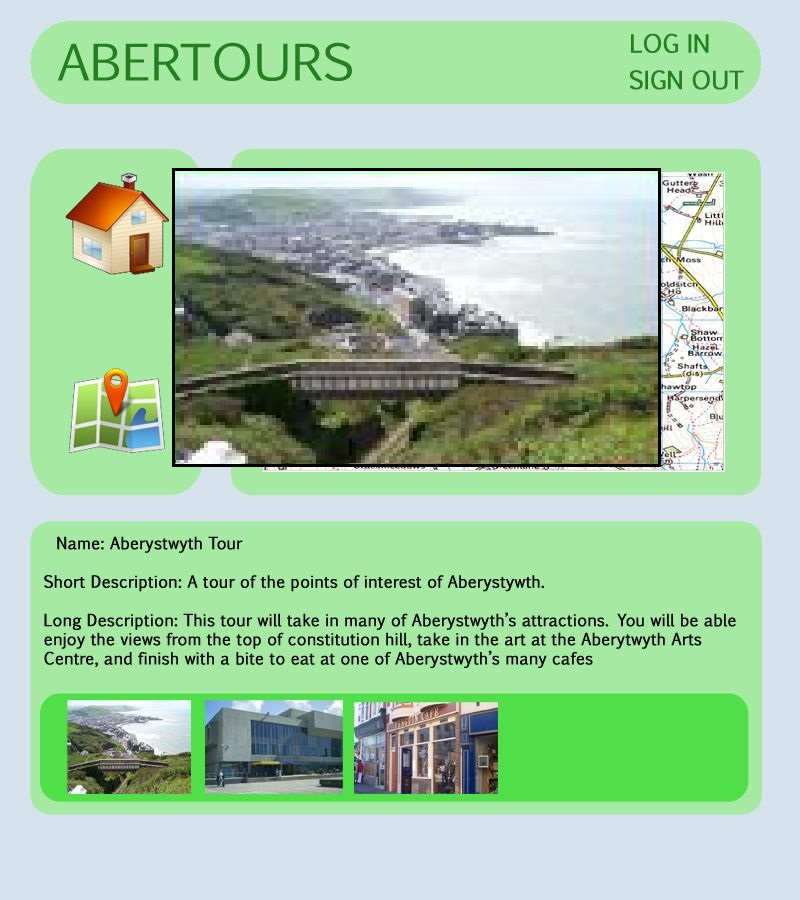
\includegraphics[scale=0.50]{Project_Plan/Web/walk_image_clicked_01.jpg}
\caption{Clicking an Image associated with a walk}
\label{Clicking an Image associated with a walk}
\end{figure}
\par{This simply enlarges the image clicked. Clicking outside the box minimizes the image back into the tray. \\ \\}
\textbf{\uline{NAVIGATION}}
\par{Click Outside Image $\rightarrow$ Previous Page}
\newpage
\section{NAVIGATION OVERVIEW}
\subsection{Android}
\begin{figure}[htp]
\begin{adjustwidth}{-3.cm}{-4cm}
\centering
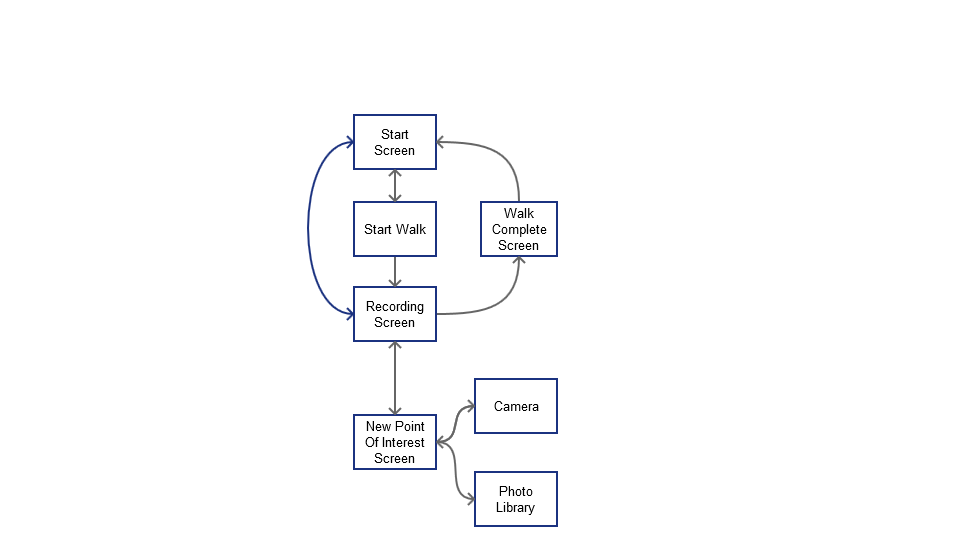
\includegraphics[scale=0.6]{Project_Plan/docs/android_navigation_01.png}
\caption{Android Navigation}
\label{Android Navigation}
\end{adjustwidth}
\end{figure}
\par{Start screen is the entry point. All navigation is done via buttons and icons unless otherwise stated}
\clearpage
\subsection{Website}
\begin{figure}[htp]
\begin{adjustwidth}{-3cm}{-3cm}
\centering
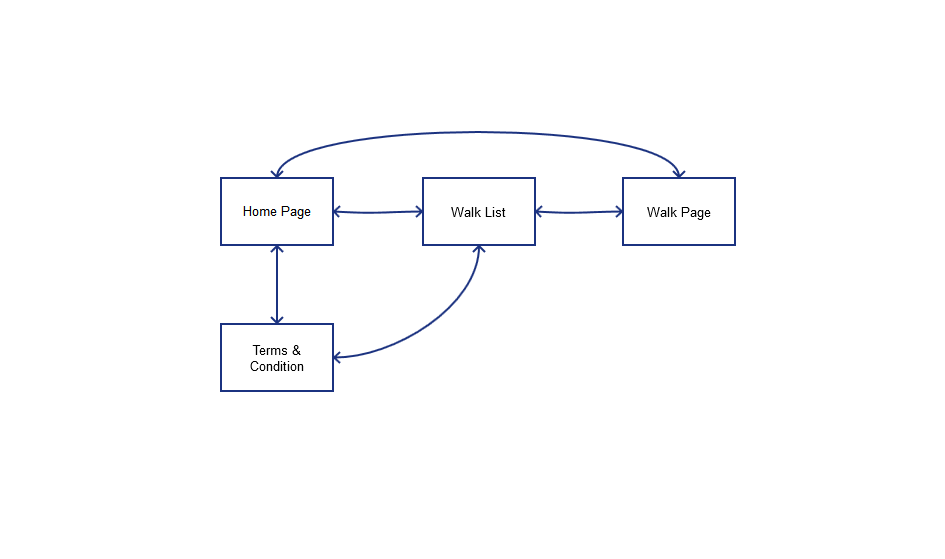
\includegraphics[scale=0.6]{Project_Plan/docs/website_navigation_01.png}

\caption{Website Navigation}
\label{Website Navigation}
\end{adjustwidth}
\end{figure}

\par{Home page is the entry point. All pages link back to the home page}
\newpage
\section{GANTT CHART}
\newgeometry{top=1.5cm, bottom =1.2cm}
\begin{landscape}
	\begin{figure}[htp]
	\begin{adjustwidth}{-0.7cm}{0cm}
\centering
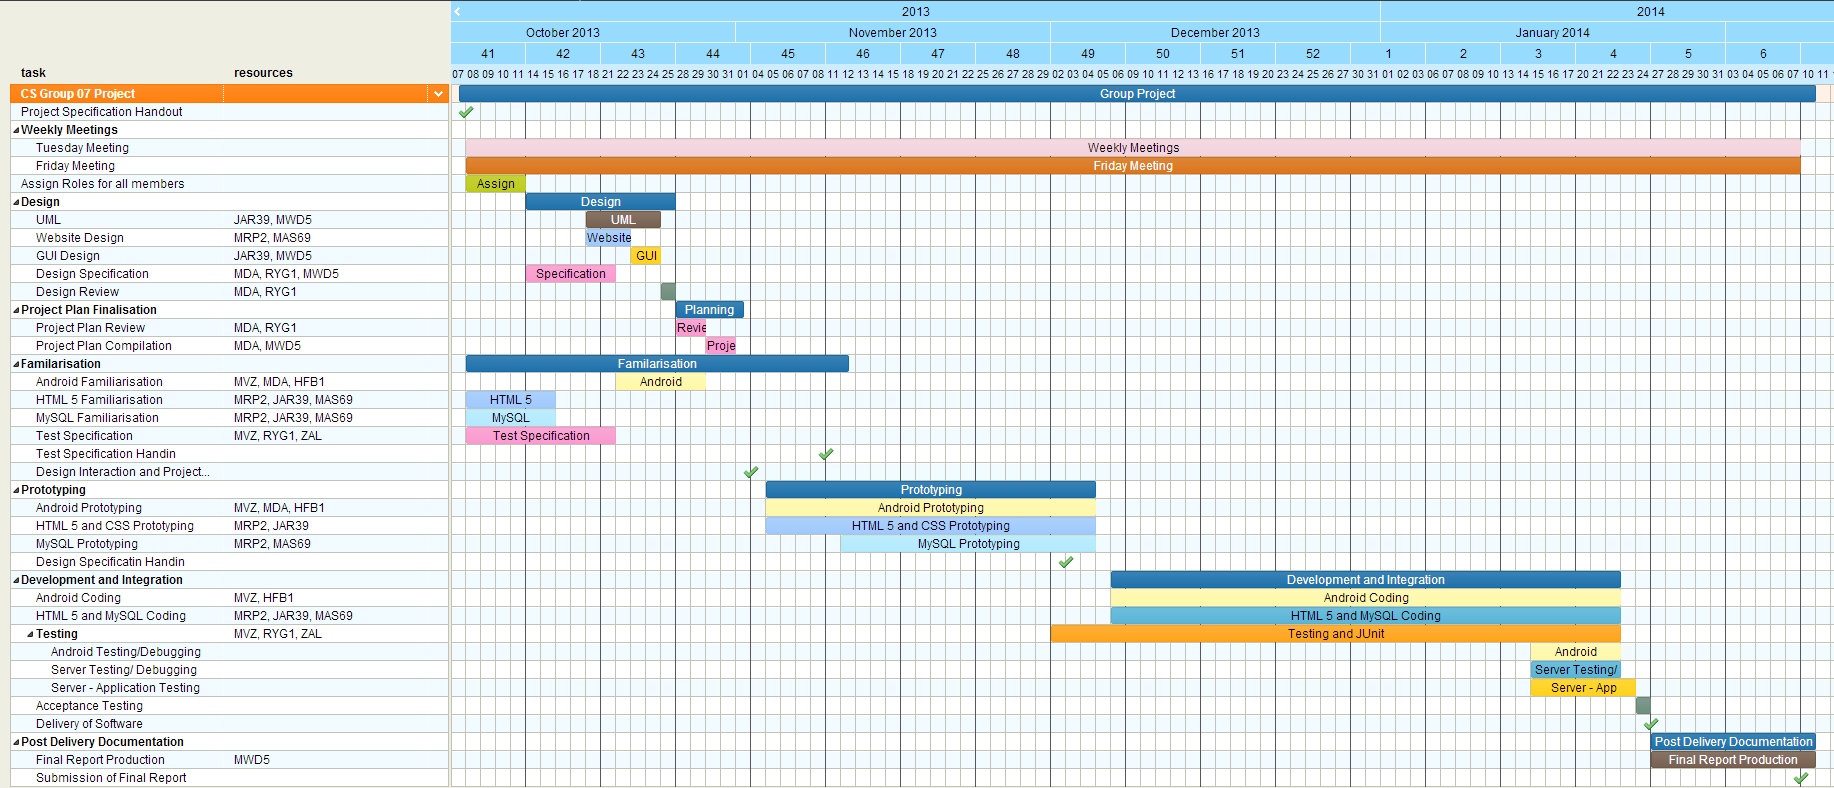
\includegraphics[scale=0.58]{Project_Plan/docs/gant_chart_01.PNG}
\caption{Gantt Chart}
\label{Gantt Chart}
\end{adjustwidth}
\end{figure}
\end{landscape}
\restoregeometry
\newpage
\section{RISK ASSESSMENT}
\begin{longtable}{|p{2.5cm}|p{1.5cm}|p{10cm}|}
\hline
	Event & Risk & Mitigation\\
\hline
	Git Downtime & Low & All work should be backed up on multiple devices, preferably the University of Aberystwyth M: Drive and local backup locations. Work can continue on local bramches\\
\hline
	Absence of Team Leader & Low & The deputy team leader will take up responsibilities as required.\\
\hline
	QA Manager Absence & Low & Team leader or deputy team leader will take up responsibilities as required. \\
\hline 
	Poor Quality Work & Low & All work must be verified and monitored by both the QA Manager and the Team Leader. Deadlines for tasks are given before official deadlines to provide a window in which work is brought up to standard. \\ 
\hline
	Problems with Maps API & Medium & In the event of inability to use the OpenSpace API, Google Maps API will be used due to its wide use. \\ 
\hline 
	Absence of Team Member & Medium & 
In the absence of any member, work will proceed as normal. All members should notify the group leader if they will be absent at the next meeting. Any absent member should read the minutes of the last meeting and any other documents produced. Continued unauthorized absence will result in warnings then penalties.\\
\hline 
	Project Off Schedule & Medium & Members are required to stick to the schedule and provide weekly reports on all project related tasks throughout the week. In the event of failure to stick to the schedule, tasks must be revised to bring project back on schedule.\\
\hline 
	Server Downtime & Medium & Website and server development should be done locally and added to the university server regularly. In the event of downtime, work should proceed as normal locally. A local LAMP or similar server may be used for testing \\
\hline 
	Unrequired Features & Medium & Extra features should not be a priority and should not be added unless the final product meets the required specification. A copy of the final product must be used for adding any extra features. \\
\hline 
	Lack of knowledge of platforms & Medium & In the event of any team member being unable to do work due to not knowing how to perform a task on the platform, the team leader must be notified. Any members capable who know how to proceed will be assigned to performing that task. All members are required to gain as much knowledge about the API and languages during the familiarisation stage. \\
\hline 
	Member Unable to Continue Project & High & If for any reason a member is unable to continue the project, tasks will be reshuffled to accommodate the change. Multiple members are assigned similar tasks to help reduce the risk in such an event. \\
\hline
	Loss of Data & High & Users are required to regularly backup data. If for any reason data is not backed up and is lost, the group leader must be notified immediately and more work must be done to bring the project back on schedule. Tasks may be reprioritised to ensure deadlines are met. \\
\hline 
	Change in Requirements & High & If requirements are changed by the client, a meeting will be called immediately to meet the new requirements. Regular communication between the client and the team leader is required. \\
\hline 
	Hardware Incompatibility & High & The application must be thoroughly tested on at least 2 android mobile devices. Tablet compatibility is not required. In the event of hardware incompatibility or related issues, extensive debugging and testing must be done and the team leader must be notified immediately. \\ 
\hline 
	Application – Server Incompatibility & High & The application should send data in the format specified. The server must be able to parse the data accurately. In the event of incompatibility, android and server side debugging must be done to determine the cause of the incompatibility. \\
\hline
\end{longtable}
\newpage
\section{DOCUMENT HISTORY}
\begin{longtable}{|p{1.5cm}|p{1.5cm}|p{2cm}|p{6cm}| p{2cm}|}
\hline
	Version & CFF No. & Date & Section Changed From Previous Version & Changed by \\
\hline
	1.0 & N/A & 28/10/13 & Original draft of document written by Mosopefoluwa David Adejumo & MDA \\ 
\hline
	1.1 & N/A & 31/10/13 & Added new screens. Updated project overview &MDA \\
\hline
	1.2 & N/A & 31/10/13 & Updated Android user interface & MDA \\
\hline 
	1.3 & N/A & 2/11/13 & Updated Android user interface and description.
Added Website User Interface Description
Added Gantt chart. Added Navigation overview
Updated risk assessment & MDA \\
\hline 
	1.4 & N/A & 2/11/13 & Added use case and descriptions. Added system overview. Updated project overview & MDA \\
\hline 
	1.5 & N/A & 2/11/13 & Updated system overview. Updated use case. Updated UI descriptions & MDA \\
\hline
	1.6 & N/A & 3/11/13 & Updated Fig. 5.3 and Fig 5.4 images. Added interaction system diagram and description.
Moved risk assessment to item 8 & MDA \\
\hline 
	1.7 & N/A & 4/11/13 & Updated Interaction System and replaced image. Corrected config ref number & MDA \\
\hline 
	1.8 & N/A & 6/11/13 & Updated Gantt chart. & MDA \\
\hline	
	1.9 & N/A & 13/02/14 & Re-wrote the document in LaTeX. & RYG1 \\
\hline
	2.0 & N/A & 13/02/14 & Added updated images to file & RYG1 \\
\hline
	2.1	& N/A & 15/02/14 & Re-sized the Gantt Chart & RYG1 \\
\hline
	2.2	& N/A & 16/02/14 & Edited Feature creep Images & RYG1 \\
\hline
	2.3	& N/A & 16/02/14 & Updated navigation and interface description texts and use case descriptions. Added system interaction diagram & MDA \\
\hline
\end{longtable}


\end{document}